\documentclass[a3paper,8pt]{extarticle}
% \usepackage[utf8]{inputenc}
\usepackage[mathletters]{ucs}
\usepackage[utf8x]{inputenc}

\usepackage{fancyhdr}

\usepackage[pdftex]{graphicx} % Required for including pictures
\usepackage[pdftex,linkcolor=black,pdfborder={0 0 0}]{hyperref} % Format links for pdf
\usepackage{calc} % To reset the counter in the document after title page
\usepackage{enumitem} % Includes lists

\usepackage{textcomp}
\usepackage{eurosym}

\usepackage{ dsfont } % font za množice
% tabele
\usepackage{array}
\usepackage{wrapfig}

\usepackage{tikz,forest}
\usetikzlibrary{arrows.meta}

\frenchspacing % No double spacing between sentences
\setlength{\parindent}{0pt}
\setlength{\parskip}{0.1em}

\usepackage{mathtools}
\usepackage{blkarray, bigstrut} %


\usepackage{amssymb,amsmath,amsthm,amsfonts}
\usepackage{multicol,multirow}
\usepackage{calc}
\usepackage{ifthen}
\usepackage{tabularx}
\usepackage[landscape]{geometry}
\usepackage{listings}
\usepackage{inconsolata}
%\usepackage[colorlinks=true,citecolor=blue,linkcolor=blue]{hyperref}
%\usepackage{accents}
\usepackage{pdfpages}

\newcommand{\vect}[1]{\accentset{\rightharpoonup}{#1}}

\ifthenelse{\lengthtest { \paperwidth = 11in}}
    { \geometry{top=.5in,left=.5in,right=.5in,bottom=.5in} }
	{\ifthenelse{ \lengthtest{ \paperwidth = 297mm}}
		{\geometry{top=1cm,left=1cm,right=1cm,bottom=1cm} }
		{\geometry{top=1cm,left=1cm,right=1cm,bottom=1cm} }
	}
\pagestyle{empty}
\makeatletter
\renewcommand{\section}{\@startsection{section}{1}{0mm}%
                                {-1ex plus -.5ex minus -.2ex}%
                                {0.5ex plus .2ex}%x
                                {\normalfont\large\bfseries}}
\renewcommand{\subsection}{\@startsection{subsection}{2}{0mm}%
                                {-1explus -.5ex minus -.2ex}%
                                {0.5ex plus .2ex}%
                                {\normalfont\normalsize\bfseries}}
\renewcommand{\subsubsection}{\@startsection{subsubsection}{3}{0mm}%
                                {-1ex plus -.5ex minus -.2ex}%
                                {1ex plus .2ex}%
                                {\normalfont\small\bfseries}}
\makeatother
\setcounter{secnumdepth}{0}
%\setlength{\parindent}{0pt}
%\setlength{\parskip}{0pt plus 0.5ex}

% listings okolje za psevdo kodo
\lstnewenvironment{koda}[1][] %defines the algorithm listing environment
{   
    \lstset{ %this is the stype
        mathescape=true,
        basicstyle=\scriptsize, 
		columns=flexible,
        keywordstyle=\bfseries\em,
        keywords={,vhod, izhod, zacetek, konec, koncamo, ponavljaj, dokler, ce, vrni, za, vsak, vse, v, sicer, alg, def} %add the keywords you want, or load a language as Rubens explains in his comment above.
        xleftmargin=.1\textwidth,
		tabsize=4,
		%frame=leftline,xleftmargin=5pt,xrightmargin=5pt,framesep=5pt,
		%inputencoding = utf8,
		extendedchars = true,
		literate={ž}{{\ˇz}}1 {š}{{\ˇs}}1 {č}{{\ˇc}}1 {Ž}{{\ˇZ}}1 {Š}{{\ˇS}}1 {Č}{{\ˇC}}1,
        #1 % this is to add specific settings to an usage of this environment (for instnce, the caption and referable label)
    }
}
{}
% -----------------------------------------------------------------------
\begin{document} 

\begin{multicols}{4}
\setlength{\premulticols}{1pt}
\setlength{\postmulticols}{1pt}
\setlength{\multicolsep}{1pt}
\setlength{\columnsep}{2pt}

\section{Uporabne formule}
\[ H_n = \sum_{k=1}^n \frac{1}{k}\; \leq \; 1 + O(\log n)\]

\[
    \begin{aligned}
        \sum_{n=0}^{\infty} q^n &= \frac{1}{1-q} &
        \sum_{n=0}^{b} q^n &= \frac{1-q^{b+1}}{1-q}
        \\
        \sum_{n=a}^{\infty} q^n &= \frac{q^{a}}{1-q} &
        \sum_{n=a}^{b} q^n &= \frac{q^a-q^{b+1}}{1-q}
    \end{aligned}
\]

\[
    a^n - b^n = (a-b)(a^{n-1} + a^{n-2}b + ... + ab^{n-2} + b^{n-1})  
\]
\[ (x+y)^n = \sum_{k=0}^{n} \binom{n}{k} x^{n-k}y^{k} \]
\[ \frac{1}{(1-x)^n} = \sum_{k=0}^{n} \binom{n+k-1}{k} x^{k} \]

\[\binom{n}{k} = \frac{n^{\underline{k}}}{k!} = \frac{n!}{k!(n-k)!} = \binom{n}{n-k}\]

\[P(A|B) = \frac{P(A\cap B)}{P(B)} \qquad P(A|B) = \frac{P(B|A)P(A)}{P(B)}\]

\subsubsection{Izbori}
Imamo $n$ oštevilčenih kroglic. Na koliko načinov lahko izberemo $k$ kroglic?

\begin{center}
    \begin{tabular}{ m{6em} | c | c | } 
         & \textbf{s pon.} & \textbf{brez pon.}\\ 
        \hline
        \textbf{variacije} \emph{vrstni red je pomemben} & $n^k$ & $n^{\underline{k}}$ \\ 
        \hline
        \textbf{kombinacije} \emph{vrstni red ni pomemben} & $\binom{n+k-1}{k}$ & $\binom{n}{k}$ \\ 
    \end{tabular}
\end{center}

\section{Verjetnostni algoritmi za odločitvene probleme}
Odgovarjamo na vprašanje $\omega \in \Pi$? \\
\textbf{Las Vegas} algoritmi vedno vrnejo pravilen odgovor \\
\textbf{Monte Carlo} algoritmi lahko vrnejo napačen odgovor
\begin{itemize}
	\item tip 1: $P(\text{yes}\ |\ \omega \in \Pi) \geq \frac{1}{2}$ $P(\text{yes}\ |\ \omega \notin \Pi) = 0$ 
	\item tip 2: $P(\text{yes}\ |\ \omega \in \Pi) = 1$ $P(\text{yes}\ |\ \omega \notin \Pi) \leq \frac{1}{2}$
	\item tip 3: $P(\text{yes}\ |\ \omega \in \Pi) \geq \frac{3}{4}$ $P(\text{yes}\ |\ \omega \notin \Pi) \leq \frac{1}{4}$
\end{itemize}

\subsubsection*{Razredi kompleksnosti odločitvenih problemov}
\begin{itemize}
	\item RP (randomized polynomial time): \\
	$\exists$ Monte Carlo tipa 1, ki v najslabšem primeru deluje v polinomskem času.
	\item co-RP: \\ 
	$\exists$ Monte Carlo tipa 2, ki v najslabšem primeru deluje v polinomskem času.
	\item BPP (bounded-error probabilistic polynomial time): $\exists$ Monte Carlo tipa 3, ki v najslabšem primeru deluje v polinomskem času.
	\item ZPP (zero-error probabilistic polynomial time): \\ 
	$\exists$ Las Vegas algoritem, ki deluje v pričakovanem polinomskem času. \\
	Ali (ekvivalentna definicija): $\exists$ alg, ki v najslabšem primeru deluje v polinomskem času in vedno vrne pravilen odgovor ali "ne vem" in $P(\text{"ne vem"}) < \frac{1}{2}$.
\end{itemize}

$\text{ZPP} = \text{RP} \cap \text{co-RP}$,\ \ $\text{P} \subset \text{ZPP}$,\ \ $\text{RP} \cup \text{co-RP} \subset \text{BPP}$

\section{Neenakost Chernoffa}
$X_1, \dots, X_n$ neodvisne slučajne spremenljivke, $X_i \in \{0, 1\}$, $X = \sum_{i=1}^n X_i$, $\mu = E(X)$. Potem za vsak $\delta \in (0,1)$ velja:

\begin{align*}
	P(X - \mu \geq \delta \mu) &\leq e^{-\frac{\delta^2 \mu}{2+\delta}} \leq e^{-\frac{\delta^2 \mu}{3}} \\
	P(\mu - X \geq \delta \mu) &\leq e^{-\frac{\delta^2 \mu}{2}} \leq e^{-\frac{\delta^2 \mu}{3}} \\
	P(|X - \mu| \geq \delta \mu) &\leq 2e^{-\frac{\delta^2 \mu}{3}} \\
\end{align*}

\section{Verjetnostni algoritmi za aproksimacijo}
Verjetnostni algoritem izračuna $(\epsilon, \delta)$-aproksimacijo za $V$, če vrne $X$ tako, da velja:
\[ P(|X-V| \leq \epsilon V ) \geq 1 - \delta \]

Naj bodo $X_1, \dots X_m$ slučajne spremenljivke, $\mu = E(X_i)$, $Y = \frac{\sum X_i}{m}$. 
Če je $m \geq \frac{3\ln(2/\delta)}{\epsilon^2 \mu}$, potem velja:
\[ P(|X-\mu| \geq \epsilon \mu) \leq \delta\]

in $Y$ je $(\epsilon, \delta)$-aproksimacija za $\mu$.

\section{Polinomi}
Naj bo $\mathbb{F}$ polje. Stopnja polinoma $p \in \mathbb{F}[x_1, \dots, x_n]$ je $\deg(p(x_1, \dots, x_n)) = \deg(p(x, \dots, x))$

\subsubsection{Predstavitev s polinomi}

\begin{align*}
    \text{\tiny terka} && T = (a_0, \dots, a_n) &\ \mapsto \ p_T(x) = \sum_{i=0}^n a_i x^i \\
    \text{\tiny terka alternativa} && T = (a_0, \dots, a_n) &\ \mapsto \ p_T(x_0, \dots, x_n) = \sum_{i=0}^n a_i x_i \\
    \text{\tiny množica} && M = \{a_0, \dots, a_n\} &\ \mapsto \ p_M(x) = \prod_{i=0}^n (x - a_i) \\
    \text{\tiny množica terk} && \{ T_0, \dots, T_m \} &\ \mapsto \ p(x,y) = \prod_{i=0}^m (y - p_{T_i}(x)) \\
    \text{\tiny množica množic} && \{ M_0, \dots, M_m \} &\ \mapsto \ p(x,y) = \prod_{i=0}^m (y - p_{M_i}(x))
    % \{(a_{00} \dost, a_{0n}), \dots, (a_{m0}, \dots, a_{mn})\} & 1
\end{align*}

Želimo ugotoviti ali je $A = B$. Skonstruiramo polinoma $p_A$ in $p_B$.
\begin{koda}
za $i = 0, \dots, k$
    $r \leftarrow$ nakljucna vrednost iz $S^n$
    ce $p_A(r) \neq p_B(r)$:
        vrni NE
vrni DA
\end{koda}
\[P(\text{DA} | A \neq B) \leq \left(\frac{d}{|S|}\right)^k\]

\subsubsection{Schwartz-Zippelov izrek}
Naj bo $p \in \mathbb{F}[x_1, \dots, x_n]$ in $\deg(p) = d \geq 0$. Naj bo $S \subseteq \mathbb{F}$ poljubna končna podmnožica. Za naključno izbiro (enakomerno) $r \in S^n$ velja:
\[ P(p(r) = 0) \leq \frac{d}{|S|} \]

\section{Verjetnost}
\textbf{Verjetnost} na $(\Omega, \mathcal{F})$ je preslikava $P: \mathcal{F} \to \mathbb{R}$ z lastnostmi:

\begin{itemize}
    \item $P(A) \geq 0$ za $\forall A \in \mathcal{F}$
    \item $P(\Omega) = 1$
    \item Za paroma nezdružljive (disjunktne) dogodke $\{ A_i \}_{i=1}^\infty $ velja \textit{števna aditivnost}
    \[ P(\bigcup_{i=1}^\infty A_i) = \sum_{i=1}^\infty P(A_i)\]
    \item $P(\emptyset) = 0$
    \item $P$ je končno aditivna.
    \item $P$ je \textit{monotona}: $A \subseteq B \implies P(A) \leq P(B)$
    \item $P(A^\complement) = 1 - P(A)$
    \item $P$ je \textit{zvezna}:
    \[ A_1 \subseteq A_2 \subseteq \dots \implies P\big(\bigcup_{i=1}^\infty\big) = \lim_{i \to \infty} P(A_i)\]
    \[ B_1 \supseteq B_2 \supseteq \dots \implies P\big(\bigcap_{i=1}^\infty\big) = \lim_{i \to \infty} P(B_i)\]
\end{itemize}

\subsection{Matematično upanje}
Za slučajno spremenljivko $X: \Omega  \to \mathbb{Z}$
\[ E(X) =  \sum_{c\in \mathbb{Z}} c P(X = c)\]

\subsubsection{Lastnosti}
\[ E(f(X)) = \sum_{c \in \mathbb{Z}} f(c) P(X = c) \]

\textit{Linearnost}: za poljubne sl. sprem $X_1, \dots, X_n$ velja:
\[ E(a_1 X_1 + \dots a_n X_n) = a_1 E(X_1) + \dots + a_n E(X_n) \]

Če ima $|X|$ mat. up., ga ima tudi $X$ in velja 
\[|E(X)| \leq E(|X|) \]

Če obstaja $E(X^2)$ in $E(Y^2)$, obstaja tudi $E(XY)$ in velja:
\[|E(XY)| \leq E(|XY|) \leq \sqrt{E(X^2)E(Y^2)} \]

\subsection{Disperzija (varianca)}
\[D(X) = E((X - E(X))^2) = E(X^2) - (E(X))^2\]
Lastnosti: 
\begin{itemize}
    \item $D(X) \geq 0$
    \item $D(X) = 0 \iff P(X = E(X)) = 1$
    \item $D(aX) = a^2 D(X)$
\end{itemize}

Standardna diviacija/odklon:
\[ \sigma(X) = \sqrt{D(X)} \]
zanjo velja $\sigma (aX) = |a|\sigma(X)$.

\subsection{Neodvisnost}
Diskretno porazdeljeni sl. sprem. $X$ in $Y$ sta noedvisni, če velja:
\[ P(X = x_i, Y = y_j) = P(X = x_i)P(Y = y_j)\]
za vse $i, j$.

\subsection{Nekoreliranost}
Sl. sprem. $X$ in $Y$ sta nekorelirani, če velja:
\[ E(XY) = E(X)E(Y) \]
\[ X, Y \text{ neodvisni } \implies X,Y \text{ nekorelirani }\]

Če imata $X$ in $Y$, je nekoreliranost ekvivalentna zvezi:
\[ D(X+Y) = D(X) + D(Y)\]


\subsection{Neenakost Markova}
Če je $X$ ne negativna sl. sprem. z mat. up., potem je
\[P(|X| \geq a) \leq \frac{E(|X|)}{a} \quad \forall a > 0\]

\subsection{Neenakost Čebiševa}
Če ima $X$ disperzijo, je
\[ P(|X - E(X)| \geq a \sigma(X)) \leq \frac{1}{a^2}  \quad \forall a > 0\]
oziroma za $\varepsilon := a \sigma(X)$
\[ P(|X-E(X)| \geq \varepsilon) \leq \frac{D(X)}{\varepsilon^2}\]

\section{Znani problemi}
\subsection{Perfect matching}
Naj bo $G$ graf. Popolno ujemanje je podmnožica povezav $M \subseteq E(G)$, tako da vejla
\begin{align*}
    \forall e, f \in M\ :\ e \cap f = \emptyset \quad \text{in} \quad
    \bigcup_{e \in M} e = V(G)
\end{align*}

$G$ imam popolno ujemanje $\iff$ $\det(A_G) \neq 0$
\begin{align*}
    A_G = [a_{ij}]_{i,j = 1}^n \qquad a_{ij} = \begin{cases}
        x_ij & \text{če } ij \in E(G), i < j \\
        -x_ij & \text{če } ij \in E(G), i > j \\
        0 & \text{sicer}
    \end{cases}
\end{align*}


\subsection{Min/max prerez (Min/max cut)}
Naj bo $G$ graf. Prerez je particija $V(G)$ na $U$ in $V(G) \setminus U$ tako da se minimizira/maksimizira število povezav med $U$ in $V(G) \setminus U$.

\begin{koda}
alg rand_min_cut
vhod: graf $G$
$G_0 \leftarrow G$
$i \leftarrow 0$
dokler $V(G_i) > 2$:
    $e \leftarrow$ nakljucna povezava v $G_i$
    $G_{i+1} \leftarrow G_i \setminus e$  // skrcitev povezave $e$ 
    $i \leftarrow i + 1$
${u,v} \leftarrow V(G_{n-2})$ // $n = |V(G)|$
$U = \{w \in V(G)\ |\ w \text{ je bil skrcen v } u \}$
vrni $(U, V(G) \setminus U)$
\end{koda}

Algoritem \texttt{rand\_min\_cut} vrne min. prerez z verjetnostjo $\frac{2}{n(n-1)}$.

\section*{Markovske verige}
\begin{align*}
    \Omega \quad &\dots \quad \text{mnočica stanj} \\
    X_t \quad &\dots \quad \text{stanje v času $t$}
\end{align*}

Markovska veriga je zaporedje slučajnih spremenljivk $X = X_0, X_1, \dots$ za katere velja, da je verjetnost prehoda odvisna le od trenutnega stanja:
\begin{multline*}
    P(X_{i+1} = x | X_0 = x_0, X_1 = x_1, \dots, X_i = x_i) = \\
    = P(X_{i+1} = x | X_i = x_i)
\end{multline*}

Lahko zahtevamo še, da je verjetnost prehoda neodvisna od časa (\textit{time homogeneous}):
\[ P(X_i+1 = x | X_i = y) = P(X_1 = x | X_0 = y)\]

Od zdaj naprej se bomo osredotočili na končno množico stanj $\Omega = \{x_1, \dots, x_n\}$. 
\begin{align*}
    \mathbf{P} = \begin{bmatrix}
        p_{ij}
    \end{bmatrix}_{i,j = 1}^n\quad &\dots \quad \text{prehodna matrika} \\
    p_{ij} \quad &\dots \quad \text{verjetnost prehoda iz $x_i$ v $x_j$}
\end{align*}

Porazdelitev stanj v času $t$:
\[q(t) = \begin{bmatrix}
    q_1(t) & \dots & q_n(t)
\end{bmatrix} \quad P(X_t = x_i) = q_i(t) \] 

velja
\[ q(t) = q(t-1) \mathbf{P} = q(0) \mathbf{P}^t \]

\subsection*{Stacionarna porazdelitev}
$\pi = \begin{bmatrix} \pi_1 \dots \pi_n \end{bmatrix}$ je stacionarna porazdelitev, če velja 
\[\pi \mathbf{P} = \pi \qquad \sum_{i} \pi_i = 1 \]

Oznake:
\begin{itemize}
    \item $f_{i,j}$ verjetnost da $X_t = x_j$ za nek (dovoj velik) $t$, če je $X_0 = x_i$
    \item $h_{i,j}$ pričakovano število korakov, da pridemo iz stanja $x_i$ v stanje $x_j$. (\textit{hitting time})
    \item $N(i, t, q(0))$ pričakovano število obiskov stanja $x_i$ po $t$ korakih, če je začetna porazdelitev $q(0)$.
\end{itemize}

Markovska veriga je \textit{irreducible} $\iff$ $\forall i, j \ f_{ij} > 0$. Za take verige velja:
\begin{itemize}
    \item $\exists$ enoloično določena stacionarna porazdelitev
    \item $f_{i,i} = 1$ in $h_{i,i} = \frac{1}{\pi_i}$
    \item $\lim_{t \to \infty} \frac{N(i, t, q(0))}{t} = \pi_i$
\end{itemize}

Markovska veriga je \textit{aperiodična}, če $\nexists c \in \{2, 3, \dots\}$, ki deli vse dolžine ciklov (v grafu prehodov med stanji). Za take verige velja še:
\begin{itemize}
    \item $\lim_{t \to \infty} q(0)P^t = \pi$
\end{itemize}


\subsection*{Markovske verige v grafu}
$G$ povezan graf. Obravnavamo naključne sprehode kot Markovske verige.
\[ \mathbf{P} = \begin{bmatrix}
    p_{uv}
\end{bmatrix}_{u,v \in V(G)} \quad 
    p_{uv} = \begin{cases}
    \frac{1}{\deg(u)} & \text{če } uv \in E(G) \\
    0 & \text{sicer}
\end{cases}\]

Velja:
\begin{gather*}
    \pi = \begin{bmatrix}
        \pi_v
    \end{bmatrix}_{v \in V(G)} \quad
    \pi_v = \frac{\deg(v)}{2|E(G)|}  \quad
    h_{v,v} = \frac{1}{\pi_v} \\
    \forall uv \in E(G)\ :\ h_{u,v} < 2|E(G)|
\end{gather*}
Pričakovano število korakov, da obiščemo vsa vozlišča je $4(|V(G)|-1)|E(G)|$.






\end{multicols}


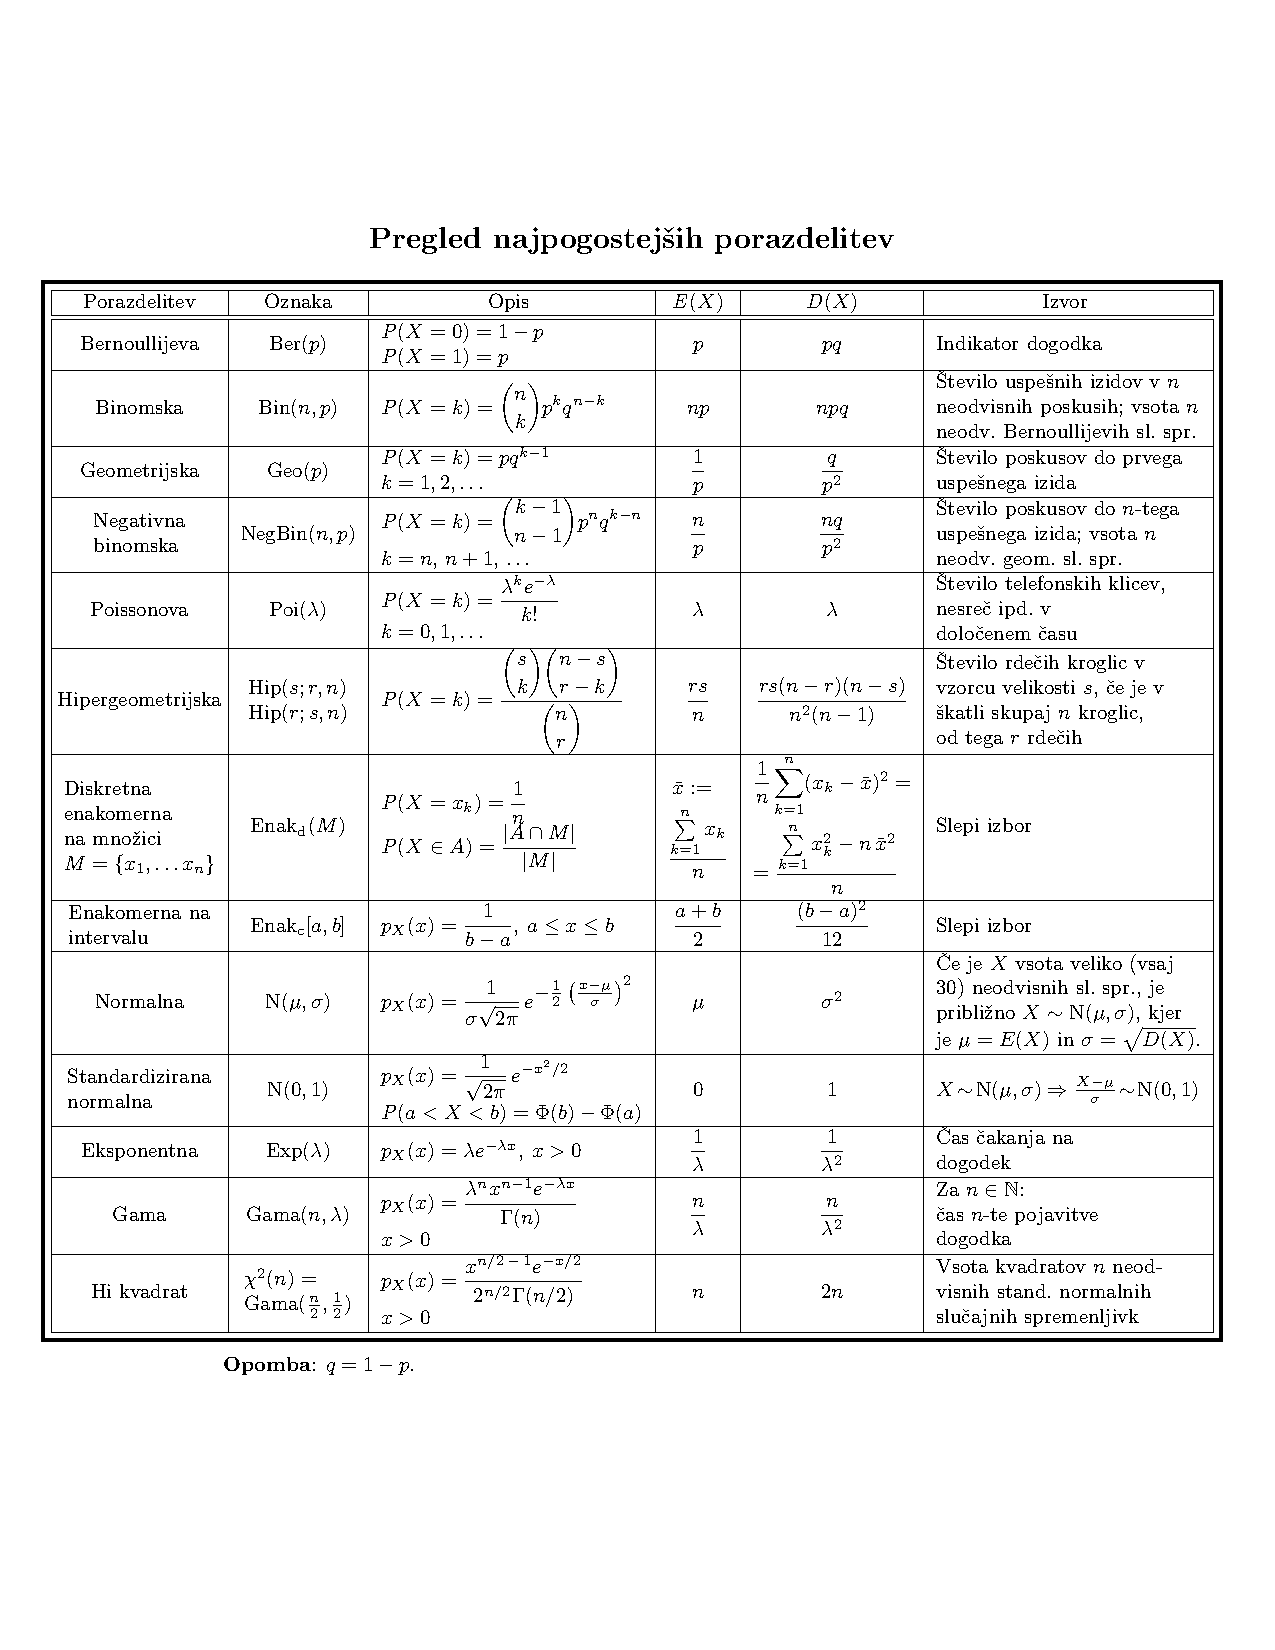
\includepdf[pages={1}]{Porazd.pdf}
\end{document}